% abtex2-modelo-artigo.tex, v-1.9.2 laurocesar
% Copyright 2012-2014 by abnTeX2 group at http://abntex2.googlecode.com/ 
%

% ------------------------------------------------------------------------
% ------------------------------------------------------------------------
% abnTeX2: Modelo de Artigo Acadêmico em conformidade com
% ABNT NBR 6022:2003: Informação e documentação - Artigo em publicação 
% periódica científica impressa - Apresentação
% ------------------------------------------------------------------------
% ------------------------------------------------------------------------

\documentclass[
	% -- opções da classe memoir --
	article,			% indica que é um artigo acadêmico
	11pt,				% tamanho da fonte
	oneside,			% para impressão apenas no verso. Oposto a twoside
	a4paper,			% tamanho do papel. 
	% -- opções da classe abntex2 --
	%chapter=TITLE,		% títulos de capítulos convertidos em letras maiúsculas
	%section=TITLE,		% títulos de seções convertidos em letras maiúsculas
	%subsection=TITLE,	% títulos de subseções convertidos em letras maiúsculas
	%subsubsection=TITLE % títulos de subsubseções convertidos em letras maiúsculas
	% -- opções do pacote babel --
	english,			% idioma adicional para hifenização
	brazil,				% o último idioma é o principal do documento
	sumario=tradicional
	]{abntex2}


% ---
% PACOTES
% ---

% ---
% Pacotes fundamentais 
% ---
\usepackage{lmodern}			% Usa a fonte Latin Modern
\usepackage[T1]{fontenc}		% Selecao de codigos de fonte.
\usepackage[utf8]{inputenc}		% Codificacao do documento (conversão automática dos acentos)
\usepackage{indentfirst}		% Indenta o primeiro parágrafo de cada seção.
\usepackage{nomencl} 			% Lista de simbolos
\usepackage{color}				% Controle das cores
\usepackage{graphicx}			% Inclusão de gráficos
\usepackage{microtype} 			% para melhorias de justificação
\usepackage{amsmath}
\usepackage{lipsum}				% para geração de dummy text
\usepackage[brazilian,hyperpageref]{backref}	 % Paginas com as citações na bibl
\usepackage[alf]{abntex2cite}	% Citações padrão ABNT
\renewcommand{\backrefpagesname}{Citado na(s) página(s):~}
\renewcommand{\backref}{}
\renewcommand*{\backrefalt}[4]{
	\ifcase #1 %
		Nenhuma citação no texto.%
	\or
		Citado na página #2.%
	\else
		Citado #1 vezes nas páginas #2.%
	\fi}%
% ---

% ---
% Informações de dados para CAPA e FOLHA DE ROSTO
% ---
\titulo{Relatório final do laboratório 01 de medição e experimentação de software}
\autor{Gabriel Nogueira Vieira Resende \and Vitor Costa Vianna \and Joaquim Guilherme de Carvalho Vilela Silva}
\local{Brasil}
\data{2026, v-1.0.0}
% ---

% ---
% Configurações de aparência do PDF final

% alterando o aspecto da cor azul
\definecolor{blue}{RGB}{41,5,195}

% informações do PDF
\makeatletter
\hypersetup{
     	%pagebackref=true,
		pdftitle={\@title}, 
		pdfauthor={\@author},
    	pdfsubject={Modelo de artigo científico com abnTeX2},
	    pdfcreator={LaTeX with abnTeX2},
		pdfkeywords={abnt}{latex}{abntex}{abntex2}{atigo científico}, 
		colorlinks=true,       		% false: boxed links; true: colored links
    	linkcolor=blue,          	% color of internal links
    	citecolor=blue,        		% color of links to bibliography
    	filecolor=magenta,      		% color of file links
		urlcolor=blue,
		bookmarksdepth=4
}
\makeatother
% --- 

% ---
% compila o indice
% ---
\makeindex
% ---

% ---
% Altera as margens padrões
% ---
\setlrmarginsandblock{3cm}{3cm}{*}
\setulmarginsandblock{3cm}{3cm}{*}
\checkandfixthelayout
% ---

% --- 
% Espaçamentos entre linhas e parágrafos 
% --- 

% O tamanho do parágrafo é dado por:
\setlength{\parindent}{1.3cm}

% Controle do espaçamento entre um parágrafo e outro:
\setlength{\parskip}{0.2cm}  % tente também \onelineskip

% Espaçamento simples
\SingleSpacing

% ----
% Início do documento
% ----
\begin{document}

% Retira espaço extra obsoleto entre as frases.
\frenchspacing 

% ----------------------------------------------------------
% ELEMENTOS PRÉ-TEXTUAIS
% ----------------------------------------------------------

%---
%
% Se desejar escrever o artigo em duas colunas, descomente a linha abaixo
% e a linha com o texto ``FIM DE ARTIGO EM DUAS COLUNAS''.
% \twocolumn[    		% INICIO DE ARTIGO EM DUAS COLUNAS
%
%---
% página de titulo
\maketitle

% resumo em português
\begin{resumoumacoluna}
A compreensão das características que definem o sucesso e a manutenção de sistemas open-source é fundamental para a engenharia de software contemporânea. Este relatório apresenta um estudo empírico baseado na mineração dos 1.000 repositórios mais populares do GitHub, avaliados pelo número de estrelas. Utilizando consultas automatizadas via API GraphQL, foram extraídas métricas referentes à idade, volume de contribuições externas (pull requests), frequência de releases, tempo de atualização, linguagens primárias e taxa de resolução de issues. Além da análise descritiva padrão, este trabalho introduz testes de hipóteses estatísticas não-paramétricas (Spearman, Mann-Whitney e Kruskal-Wallis) para validar correlações entre maturidade do projeto e engajamento da comunidade. Paralelamente à análise de dados, o documento detalha a configuração do processo de desenvolvimento da equipe, fundamentado na metodologia Kanban através do GitHub Projects, incluindo políticas de limite de Work in Progress (WIP) e rastreabilidade contínua de tarefas. 
 \vspace{\onelineskip}
 
 \noindent
 \textbf{Palavras-chaves}: Mineração de Repositórios de Software. Métricas de \textit{Software}. Código Aberto. Estatística Não-Paramétrica. Kanban.
\end{resumoumacoluna}

% ]  				% FIM DE ARTIGO EM DUAS COLUNAS
% ---

% ----------------------------------------------------------
% ELEMENTOS TEXTUAIS
% ----------------------------------------------------------
\textual

% ----------------------------------------------------------
% Introdução
% ----------------------------------------------------------
\section*{Introdução}
\addcontentsline{toc}{section}{Introdução}

Ecossistemas de código aberto são pilares da infraestrutura moderna de software. Projetos hospedados em plataformas como o GitHub não apenas democratizam o acesso a ferramentas complexas, mas também servem como laboratórios em tempo real para a observação de práticas de engenharia, governança de código e colaboração distribuída. Entender o que torna um repositório "popular" e como essa popularidade se traduz em saúde e sustentabilidade do software é um desafio constante para pesquisadores e engenheiros de plataformas.

O presente trabalho, desenvolvido no contexto da disciplina de Laboratório de Experimentação de Software, tem o duplo objetivo de executar a mineração de dados em larga escala e estabelecer um fluxo de trabalho estruturado e ágil para a equipe.

Na primeira frente, investigamos sete Questões de Pesquisa (RQs) predefinidas, analisando os 1.000 repositórios mais estrelados do GitHub para extrair e discutir métricas de maturidade, engajamento comunitário e ritmo de manutenção. Para elevar o rigor da pesquisa, estendemos a análise descritiva com o uso de métodos de inferência estatística, buscando comprovar matematicamente as correlações observadas e evitar conclusões baseadas em viés de amostragem.

Na segunda frente, documentamos a governança do próprio projeto. Adotamos o GitHub Projects (v2) como ferramenta de gestão, implementando um quadro Kanban com fluxo de estados definido, limites rigorosos de trabalho em progresso (WIP) e rastreabilidade ponta a ponta entre commits e issues. Essa estrutura garante não apenas a entrega iterativa das sprints, mas simula um ambiente de desenvolvimento profissional.
Este exemplo deve ser utilizado como complemento do manual da classe

% ----------------------------------------------------------
% Seção de Hipóteses Informais dos RQs
% ----------------------------------------------------------
\section{Hipóteses Informais}
\label{sec:hipoteses_informais}

Esta seção apresenta as respostas esperadas baseadas na intuição antes da coleta empírica de dados, cobrindo as características fundamentais dos sistemas \textit{open-source} em análise:

\begin{itemize}
    \item \textbf{RQ01 (Maturidade/Idade):} Projetos populares tendem a ser antigos. A construção de uma comunidade engajada e a consolidação de uma base de código estável exigem anos de desenvolvimento contínuo.
    
    \item \textbf{RQ02 (Contribuição externa):} Sistemas populares recebem um alto volume de \textit{pull requests}. A alta visibilidade atrai um ecossistema global de desenvolvedores dispostos a corrigir \textit{bugs} e propor \textit{features}.
    
    \item \textbf{RQ03 (Frequência de \textit{releases}):} Repositórios populares lançam \textit{releases} com alta frequência, refletindo a adoção de práticas modernas de integração e entrega contínuas (CI/CD) e a necessidade de entregar valor constante aos usuários.
    
    \item \textbf{RQ04 (Frequência de atualização):} Projetos populares são atualizados constantemente. Um baixo tempo desde a última atualização (geralmente em dias ou horas) é um indicativo de um projeto vivo e com manutenção ativa.
    
    \item \textbf{RQ05 (Linguagens populares):} A vasta maioria dos sistemas populares é escrita em linguagens consolidadas na indústria e nos \textit{rankings} globais (como Python, JavaScript, Java e C++), refletindo a demanda do mercado de \textit{software}.
    
    \item \textbf{RQ06 (Taxa de \textit{issues} fechadas):} Existe uma alta proporção de \textit{issues} fechadas em relação ao total. Isso indica uma governança técnica sólida e uma equipe de mantenedores com capacidade operacional para lidar com a demanda da comunidade.
    
    \item \textbf{RQ07 (Cruzamento de Linguagem vs. Engajamento):} Projetos escritos nas linguagens mais populares do mercado recebem mais contribuições externas e \textit{releases}, pois a barreira de entrada é menor devido à abundância de desenvolvedores fluentes nessas tecnologias.
\end{itemize}

\section{Hipóteses Extras (Testes Estatísticos)}
\label{sec:hipoteses_extras}

Para estender a análise além da estatística descritiva, formulamos hipóteses inferenciais para testar matematicamente as correlações observadas no \textit{dataset}. Dada a natureza típica das métricas de \textit{software}, que não assumem uma distribuição normal, foram selecionados testes não-paramétricos \cite{borges2016understanding}.

\subsection{Idade vs. Engajamento (RQ01 e RQ02)}
Avaliamos se o tempo de vida do repositório impacta a atração de contribuições da comunidade, utilizando o \textbf{Teste de Correlação de Spearman}.

\begin{itemize}
    \item $H_0$: Não há correlação monotônica entre a idade do repositório e o número total de \textit{pull requests} aceitos.
    \item $H_1$: Existe uma correlação monotônica positiva entre a idade do repositório e o número total de \textit{pull requests} aceitos.
\end{itemize}

\subsection{Maturidade vs. Resolução de Issues (RQ04 e RQ06)}

Verificamos se repositórios mais maduros apresentam uma proporção diferente de resolução de problemas em comparação com repositórios mais jovens, utilizando o \textbf{Teste U de Mann-Whitney}. A maturidade foi definida com base na mediana da idade dos repositórios (em dias): projetos com idade acima da mediana foram classificados como \textit{Maduros}, e os demais como \textit{Jovens}.

\begin{itemize} \item $H_0$: A mediana da razão de \textit{issues} fechadas é igual para repositórios maduros e repositórios jovens. \item $H_1$: A mediana da razão de \textit{issues} fechadas é diferente entre os dois grupos independentes. \end{itemize}


\subsection{Ecossistema de Linguagens (RQ07)}
Analisamos se a linguagem primária afeta o engajamento da comunidade de forma significativa, isolando as três principais linguagens da amostra por meio do \textbf{Teste de Kruskal-Wallis}.

\begin{itemize}
    \item $H_0$: As medianas do total de \textit{pull requests} aceitos são iguais entre as três linguagens primárias mais populares da amostra.
    \item $H_1$: Pelo menos uma das linguagens possui uma mediana de \textit{pull requests} estatisticamente diferente das demais.
\end{itemize}

\bookmarksetup{startatroot}% 

\section{Metodologia de Coleta}
\label{sec:metodologia}

Para a realização deste estudo empírico, a coleta de dados foi automatizada por meio de um \textit{script} desenvolvido pela equipe, consumindo diretamente a API GraphQL do GitHub. A consulta foi parametrizada para extrair os 1.000 repositórios com o maior número de estrelas (\textit{stars}), garantindo o foco na "elite" do ecossistema \textit{open-source}.

Para contornar os limites de paginação da API, o \textit{script} implementou requisições iterativas utilizando o sistema de cursores do GraphQL, consolidando os dados brutos em um arquivo \texttt{.csv}. 

Conforme o planejamento das \textit{Sprints}, cada membro da equipe validou individualmente o \textit{dataset} referente às suas Questões de Pesquisa (RQs). Durante esta etapa de sanitização, analisou-se a distribuição dos dados e a presença de \textit{outliers}. Optamos por \textbf{manter todos os \textit{outliers}} identificados pelo critério do intervalo interquartil (IQR), uma vez que valores extremos em métricas de repositórios populares (ex: projetos com dezenas de milhares de \textit{pull requests}) refletem fenômenos legítimos do ecossistema e não erros de coleta. A escolha por métodos estatísticos não-paramétricos, baseados na mediana e em ordenações, torna a análise robusta a esses valores extremos sem a necessidade de descartá-los. Repositórios com valores ausentes em métricas críticas (como ausência de \textit{issues} rastreáveis) foram tratados para evitar divisões por zero, garantindo a integridade dos cálculos das medianas e dos testes não-paramétricos subsequentes.

\subsection{Verificação e qualidade do software}

A implementação foi acompanhada por uma suíte automatizada de testes desenvolvida com o \textit{framework} \texttt{pytest}. Os testes verificam o cálculo das métricas das RQ01 a RQ07, incluindo casos-limite como ausência de linguagem primária, \textit{issues}, \textit{releases} ou \textit{pull requests}. A suíte também cobre o uso dos cursores na paginação da coleta de repositórios e dos itens do GitHub Projects, além da transformação dos dados do quadro e da escrita dos \textit{snapshots} em arquivos CSV. Dependências específicas de desenvolvimento são mantidas separadamente e a configuração do \texttt{pytest} define os diretórios de código e de testes utilizados pelo projeto.

Antes da exportação para CSV, cada registro coletado é validado por um modelo Pydantic, que explicita os nomes e tipos esperados para os campos das métricas e impede que registros incompatíveis com essa estrutura sejam exportados silenciosamente.


% --- SEÇÃO III: RESULTADOS POR RQ ---
\section{Resultados}
\label{sec:resultados}

A análise descritiva dos 1.000 repositórios coletados retornou os seguintes resultados numéricos para cada métrica estabelecida. Devido à natureza assimétrica dos dados de \textit{software}, adotamos a mediana como medida de tendência central.

\begin{itemize}
    \item \textbf{RQ01 (Maturidade/Idade):} A mediana de idade dos repositórios analisados é de \textbf{2.820 dias} (aproximadamente \textbf{7,73 anos}).
    \item \textbf{RQ02 (Contribuição externa):} A mediana do total de \textit{pull requests} aceitos é de \textbf{765,5}.
    \item \textbf{RQ03 (Frequência de \textit{releases}):} Os repositórios lançam, em mediana, \textbf{40} \textit{releases}.
    \item \textbf{RQ04 (Frequência de atualização):} O tempo mediano desde a última atualização até a data da coleta foi de \textbf{0 dias}, indicando que a esmagadora maioria dos repositórios populares foi atualizada no mesmo dia da coleta.
    \item \textbf{RQ05 (Linguagens populares):} As linguagens primárias mais frequentes na amostra foram: \textbf{Python} (24,97\%), \textbf{TypeScript} (19,06\%) e \textbf{JavaScript} (12,05\%).
    \item \textbf{RQ06 (Taxa de \textit{issues} fechadas):} A mediana da razão entre \textit{issues} fechadas e o total de \textit{issues} é de \textbf{87,5\%}.
    \item \textbf{RQ07 (Cruzamento de Linguagem vs. Engajamento):} Filtrando os sistemas pelas linguagens mais populares identificadas, observamos as seguintes medianas para \textit{pull requests}, \textit{releases} e dias desde a última atualização, respectivamente: \textbf{Python} (559,5 PRs; 20,5 \textit{releases}; 0 dias), \textbf{TypeScript} (1.990,5 PRs; 134 \textit{releases}; 0 dias) e \textbf{JavaScript} (630,5 PRs; 39 \textit{releases}; 0 dias).
\end{itemize}

\subsection{Visualização interativa dos resultados}

Como apoio à exploração dos dados, foi desenvolvido um \textit{dashboard} para execução local com o \textit{framework} Streamlit. A aplicação lê o arquivo CSV mais recente produzido pela coleta e apresenta indicadores gerais, medidas descritivas e gráficos das RQ01 a RQ07. A manipulação tabular é realizada com Pandas e as visualizações por linguagem utilizam Altair. O painel também exibe os resultados dos testes de Spearman, Mann--Whitney e Kruskal--Wallis, indicando se o valor-p obtido é estatisticamente significativo para o nível de 5\%. Dessa forma, o \textit{dashboard} complementa as tabelas e valores consolidados no relatório com uma forma interativa de inspecionar as distribuições e comparações entre linguagens.


% --- SEÇÃO IV: DISCUSSÃO HIPÓTESE VS. RESULTADO ---
\section{Discussão: Hipóteses vs. Resultados}
\label{sec:discussao}

Nesta seção, confrontamos as hipóteses informais preestabelecidas com os resultados descritivos, e aprofundamos a análise com os testes estatísticos inferenciais adotados.

\subsection{Análise Descritiva (RQs 1 a 7)}
\begin{itemize}
    \item \textbf{RQ01 e RQ02:} A hipótese de que projetos populares são antigos e engajados foi \textbf{confirmada}, dado que a mediana de idade é de \textbf{7,73 anos} e a mediana de \textit{pull requests} aceitos é de \textbf{765,5}, valores compatíveis com projetos consolidados e com comunidades ativas.
    \item \textbf{RQ03 e RQ04:} A expectativa de manutenção constante foi \textbf{confirmada}, observando-se um intervalo mediano de atualização de apenas \textbf{0 dias} (i.e., a maioria absoluta dos repositórios foi atualizada no mesmo dia da coleta). Além disso, a mediana de 40 \textit{releases} corrobora a adoção de práticas contínuas de entrega.
    \item \textbf{RQ05, RQ06 e RQ07:} A suposição sobre o domínio de linguagens de mercado foi \textbf{confirmada}, com liderança de \textbf{Python} (24,97\%), seguido por \textbf{TypeScript} (19,06\%) e \textbf{JavaScript} (12,05\%). A governança se mostrou \textbf{eficiente}, com \textbf{87,5\%} de taxa mediana de resolução de \textit{issues}. Ainda que a hipótese sobre linguagens de mercado tenha sido confirmada, o cruzamento da RQ07 revelou que \textit{TypeScript} apresenta a maior mediana de PRs aceitos (1.990,5), sugerindo que o domínio quantitativo não se traduz linearmente em engajamento por projeto.
\end{itemize}

\subsection{Análise Inferencial}
Para validar matematicamente as dinâmicas de engenharia de \textit{software} sugeridas, aplicamos estatística não-paramétrica \cite{borges2016understanding}:

\begin{itemize}
    \item \textbf{Idade vs. Engajamento (Spearman):} O teste de correlação de Spearman revelou $\rho = 0{,}226$ com valor-p $\approx 4{,}31 \times 10^{-13}$. Portanto, \textbf{rejeitamos} a hipótese nula, indicando que \textbf{existe} correlação monotônica positiva e estatisticamente significativa entre maturidade e volume de \textit{pull requests}. A magnitude do coeficiente ($\rho \approx 0{,}23$) sugere, contudo, uma associação de intensidade fraca a moderada: a idade contribui para explicar o engajamento, mas não é o fator dominante.
    
    \item \textbf{Maturidade vs. Resolução de \textit{Issues} (Mann-Whitney U):} Ao comparar repositórios ``Maduros'' (idade $>$ mediana) e ``Jovens'' (idade $\le$ mediana), obtivemos $U = 139.072$ com valor-p $\approx 8{,}83 \times 10^{-9}$. Isso demonstra estatisticamente que a taxa de fechamento de \textit{issues} \textbf{é diferente} entre os dois grupos. As medianas revelam a direção do efeito: repositórios maduros apresentam mediana de \textbf{0,9094}, enquanto os jovens apresentam \textbf{0,8330}, sugerindo que projetos mais antigos tendem a manter uma governança de \textit{issues} mais eficiente.
    
    \item \textbf{Linguagens vs. Engajamento (Kruskal-Wallis H):} A comparação do volume de PRs entre as três linguagens mais frequentes (Python, TypeScript e JavaScript) retornou $H = 48{,}44$ com valor-p $\approx 3{,}03 \times 10^{-11}$, evidenciando que a linguagem primária \textbf{influencia} o engajamento da comunidade de forma estatisticamente significativa. Consistentemente com a análise descritiva, TypeScript concentra a maior mediana de PRs (1.990,5) frente a Python (559,5) e JavaScript (630,5), indicando um ecossistema com padrões distintos de contribuição.
\end{itemize}


% --- SEÇÃO V: CONFIGURAÇÃO DO PROCESSO ---
\section{Configuração do Processo}
\label{sec:configuracao_processo}

Para gerenciar o fluxo de trabalho durante as \textit{sprints}, a equipe utilizou o \textit{GitHub Projects (v2)} seguindo os princípios da metodologia Kanban. 

O quadro foi estruturado com as colunas \texttt{Backlog}, \texttt{To Do}, \texttt{Doing}, \texttt{Review} e \texttt{Done}. Para garantir o foco e mitigar o acúmulo de tarefas, implementamos uma política de \textit{Work in Progress} (WIP) restrita à coluna \texttt{Doing}, permitindo um limite máximo de \textbf{3 \textit{cards}} simultâneos (correspondente a uma tarefa por membro da equipe em andamento por vez).

Para centralizar os trabalhos da disciplina, nossa equipe criou uma organização no GitHub, na qual pretende manter um repositório para cada laboratório. Essa estrutura concentra o código, as \textit{Issues}, os quadros e as permissões dos integrantes em um espaço compartilhado, em vez de vinculá-los à conta pessoal de apenas um membro.

\subsection{Revisão de código e proteção da branch principal}

A \textit{branch} \texttt{main} foi protegida contra integração direta de alterações. Toda mudança deve ser submetida por meio de uma \textit{pull request} e receber ao menos uma revisão aprovada de outro integrante. Depois da aprovação e das demais verificações obrigatórias, o \textit{merge} pode ser realizado pelo revisor ou por outro membro autorizado da organização, mas não pelo autor da \textit{pull request}. Essa revisão cruzada acrescenta uma etapa de verificação por pares e distribui entre os integrantes o conhecimento sobre as alterações incorporadas ao projeto.

\subsection{Integração contínua}

O repositório utiliza GitHub Actions para executar automaticamente a suíte de testes. O \textit{workflow} é acionado tanto em \textit{pull requests} destinadas à \texttt{main} quanto em atualizações dessa \textit{branch}; nele, um ambiente Ubuntu configura o Python 3.12, instala as dependências de desenvolvimento e executa o comando \texttt{pytest}. O resultado dessa execução é uma verificação obrigatória da \textit{pull request}: caso algum teste falhe, o \textit{merge} permanece bloqueado. A automação caracteriza uma prática de integração contínua (CI), pois valida cada alteração candidata antes que ela seja incorporada à linha principal do projeto.

A rastreabilidade foi mantida exigindo que todos os \textit{commits} do repositório mencionassem a respectiva \textit{Issue} de origem. Além disso, ao término de cada ciclo (S01, S02 e S03), o estado do quadro foi exportado para \textit{snapshots} em formato \texttt{.csv}, refletindo o fluxo real da equipe.

A Figura~\ref{fig:board-final} registra o estado final do quadro ao término do Lab01, evidenciando as colunas adotadas e a movimentação das \textit{Issues} ao longo do fluxo de trabalho.

\begin{figure}[htb]
    \centering
    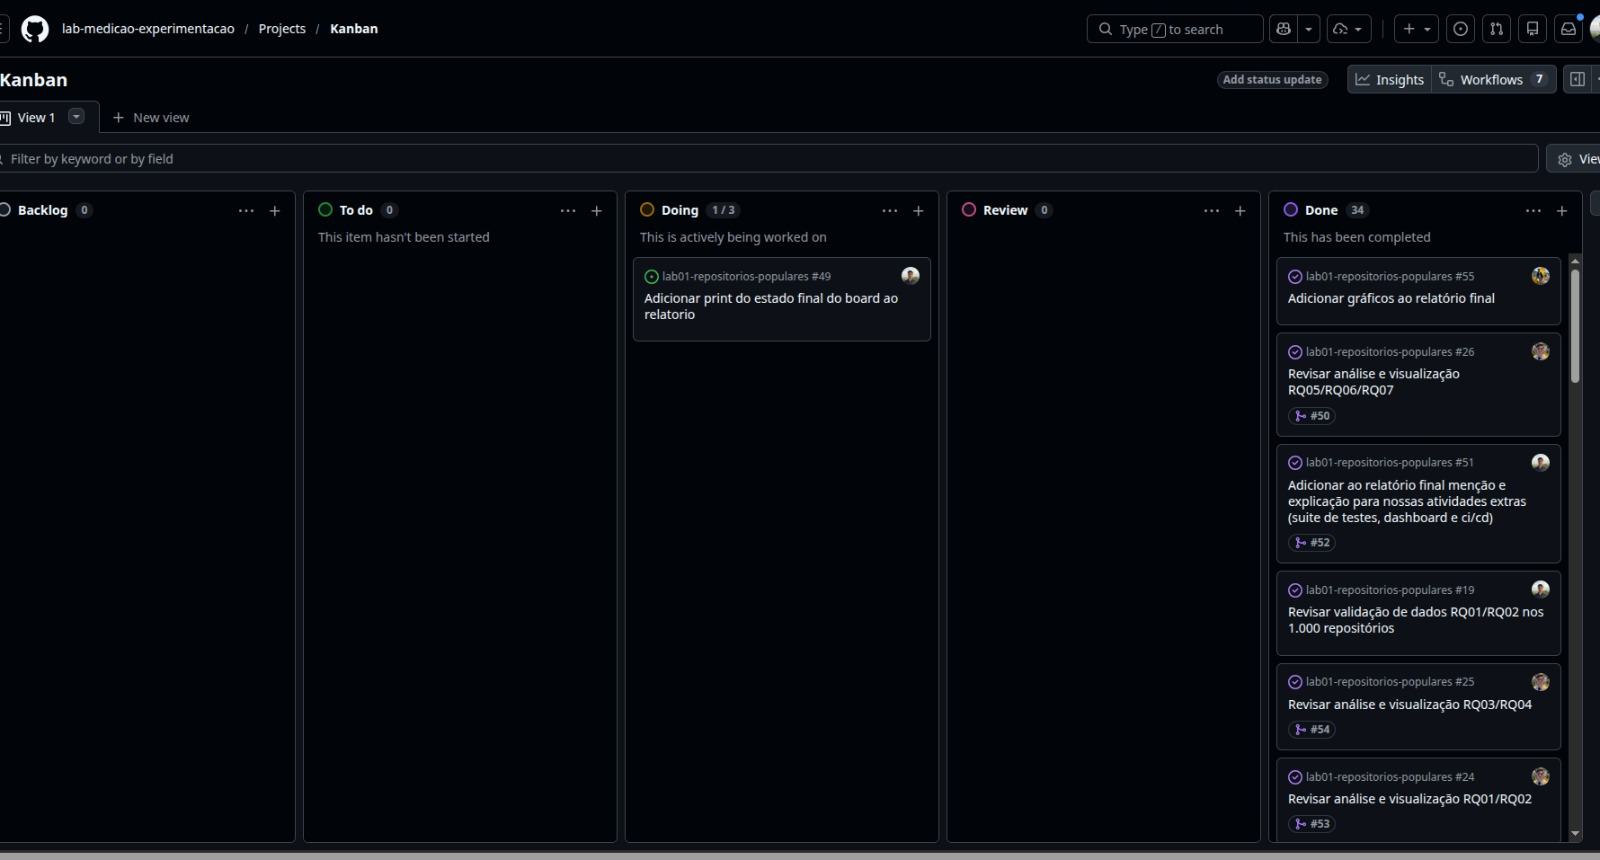
\includegraphics[width=\textwidth]{print_final_board.jpeg}
    \caption{Quadro Kanban do GitHub Projects ao final do Lab01.}
    \label{fig:board-final}
\end{figure}

\vspace{0.5cm}
\noindent \textbf{Link do Repositório (Grupo):} \url{https://github.com/lab-medicao-experimentacao/lab01-repositorios-populares}
% ---
% Conclusão
% ---
\section*{Considerações finais}
\addcontentsline{toc}{section}{Considerações finais}
Este estudo empírico investigou as características que definem a "elite" do ecossistema \textit{open-source}, analisando os 1.000 repositórios mais populares do GitHub sob a ótica de sete Questões de Pesquisa e três testes estatísticos não-paramétricos. Os resultados sustentam, em sua maioria, as intuições iniciais da equipe: repositórios populares tendem a ser maduros (mediana de 7,73 anos), altamente colaborativos (mediana de 765,5 \textit{pull requests} aceitos), ativamente mantidos (mediana de 0 dias desde a última atualização) e eficientes na governança de \textit{issues} (razão mediana de fechamento de 87,5\%).

Do ponto de vista inferencial, os três testes aplicados rejeitaram suas respectivas hipóteses nulas com significância elevada ($p < 0{,}001$). A correlação de Spearman entre idade e volume de \textit{pull requests} ($\rho = 0{,}226$) confirma uma associação positiva porém de intensidade fraca a moderada, indicando que o tempo de vida contribui para o engajamento, mas não o determina. O teste de Mann-Whitney U evidenciou que repositórios maduros mantêm uma razão de \textit{issues} fechadas significativamente maior que os jovens (0,9094 vs. 0,8330), reforçando a hipótese de que a consolidação de processos de manutenção é um resultado do amadurecimento do projeto. Por fim, o teste de Kruskal-Wallis H revelou diferenças estatisticamente significativas no volume de contribuições entre Python, TypeScript e JavaScript, com destaque para TypeScript, que apresentou a maior mediana de PRs por projeto (1.990,5), sugerindo que dinâmicas específicas de cada ecossistema exercem influência mensurável sobre o padrão de contribuição da comunidade.

Entre as limitações do estudo, destacam-se: (i) o recorte transversal da coleta, que impede análises longitudinais sobre a evolução dos repositórios; (ii) a métrica \textit{timeSinceLastUpdate} apresentou variação insuficiente na amostra (praticamente todos os repositórios foram atualizados no dia da coleta), o que exigiu adaptação da hipótese original de "Ativo vs. Dormente" para uma comparação entre "Maduros vs. Jovens"; e (iii) o critério de popularidade adotado (número de estrelas) captura visibilidade, mas não necessariamente qualidade técnica ou impacto real dos projetos.

Como trabalhos futuros, sugere-se a incorporação de séries temporais para acompanhar a trajetória dos repositórios ao longo dos anos, a inclusão de métricas de qualidade de código (cobertura de testes, complexidade ciclomática) e a análise qualitativa dos \textit{outliers} identificados, os quais frequentemente representam projetos disruptivos cujos padrões diferem da tendência central da amostra.

Paralelamente à contribuição empírica, o processo de desenvolvimento adotado, fundamentado em Kanban com limites explícitos de \textit{Work in Progress} e rastreabilidade ponta a ponta entre \textit{commits} e \textit{issues}, mostrou-se adequado ao contexto de uma equipe pequena distribuindo tarefas ao longo de \textit{sprints} curtas, e serve como referência para futuros trabalhos de mineração de repositórios conduzidos em contexto acadêmico.


%\lipsum[1]
%
%\begin{citacao}
%\lipsum[2]
%\end{citacao}
%
%\lipsum[3]




% ----------------------------------------------------------
% Referências bibliográficas
% ----------------------------------------------------------
\bibliography{references}
\end{document}
